\section{Aufgabe 1 - Anzahl von Schnittpunkten berechnen}
\label{sec:Aufgabe1}
In dieser Aufgabe soll eine Datei mit Liniensegmenten eingelesen werden und die Liniensegmente anschlie{\ss}end auf Schnittpunkte überprüft werden. Ein Liniensegment besitzt im Gegensatz zu einer Geraden einen Start- und einen Endpunkt. Diese Punkte sind je durch X- und Y-Koordinate definiert. Eine Zeile in der einzulesenden Datei enthält pro Zeile die beiden Koordinaten von Beginn und Ende des Segments. Ein Schnittpunkt ist dann vorhanden, wenn die Segmente mindestens einen gemeinsamen Punkt besitzen.

Der Algorithmus sollte zu Beginn möglichst einfach sein, deshalb wird jede Linie mit jeder anderen Linie auf einen Schnittpunkt getestet. Dadurch entsteht eine abstrakte Laufzeit von \text{O(n}\textsuperscript{2}\text{)}.

Um den Algorithmus testen zu können gab es drei verschiedene Files, die sich vorallem in der Anzahl der Input-Datensätze unterscheiden. Eine Datei beinhaltet 1000 Segmenten, die Zweite 10.000 Segmente und die Dritte 100.000 Segmente. Die tatsächliche Laufzeit verlängert sich bei Verzehnfachung des Inputs um ca. das 100 Fache.

\subsection{Einlesen der Daten}
\label{subsec:A1_EinlesenDaten}

%%FEHLT NOCH........


\subsection{Ablauf des Algorithmus}
\label{subsec:A1_Algorithmus}
Nachdem die Segmente eingelesen sind, wird die Funktion zur Berechnung der sich schneidenden Linien aufgerufen. Darin enthalten ist die Zeitmessung, diese wird direkt am Funktionsbeginn gestartet und vor der Rückgabe beendet. 

Jede Linie muss immer nur ein Mal mit jeder anderen Linie auf mindestens einen gemeinsamen Punkt getestet werden. Deshalb wird der Test in einer verschachtelten Schleife so realisiert, dass die innere Schleife immer nur nachfolgende Linien abfrägt. Doppelte Abfragen, wie Linie 3 mit Linie 4 und Linie 4 mit Linie 3, werden somit verhindert.

\begin{lstlisting}[captionpos=b, caption={Schleifenkostrukt zur Schnittpunktsuche}, label=A1:Schleife]
	for(unsigned int i = 0; i < m_lines.size(); i++) {
		for(unsigned int j = i+1; j < m_lines.size(); j++) {

			if(m_lines[i]->is_intersection(m_lines[j]) == true) {
				m_intersected_lines_nr++;
			}
		}
	}
\end{lstlisting}

Ergibt der Test auf einen Schnittpunkt ein true, wird eine Membervariable inkrementiert. Der Algorithmus terminiert wenn das Array, das die Segmente beinhaltet, komplett geprüft wurde. Das Ergebnis ist die Anzahl der Schnittpunkte und wird durch die Membervariable festgehalten.

\subsection{Test auf Schnittpunkte}
\label{subsec:A1_Schnittpunkte}

Der Test ob es einen Schnittpunkt gibt erfolgt geschachtel und wird durch die Funktion ccw\(Punkt, Punkt, Punkt\) unterstützt. Die Funktion bestimmt die Fläche, die durch die drei übergebenene Punkte aufgespannt wird. Je nach Vorzeichen der Fläche kann nun bestimmt werden, ob das Dreieck rechtsdrehend, linksdrehend oder flach ist. Flach bedeutet in diesem Fall, dass die drei Punkte auf einer Geraden liegen. Durch die Drehrichtung des Dreiecks kann bestimmt werden auf welcher Seite der Linie der dritte Punkt liegt.

\begin{lstlisting}[captionpos=b, caption={ccw-Funktion - test der Drehrichtung}, label=A1:Counterclockwise]
int Line::ccw_max(Point &a_p, Point &a_q, Point &a_r){

	//x und y koordinaten der Punkte
	double result;

	result = (a_p.get_y()*a_r.get_x())-(a_q.get_y()*a_r.get_x());
	result += (a_q.get_x()*a_r.get_y())-(a_p.get_x()*a_r.get_y());
	result += (a_p.get_x()*a_q.get_y())-(a_p.get_y()*a_q.get_x());

	if (result < 0.0)
		return -1;
	else if(result == 0.0)
		return 0;
	else
		return +1;
}
\end{lstlisting}

\subsubsection{Kolinearität}
Zuerst werden die beiden Linien auf Kolinierität geprüft, das würde bedeuten, dass kein Dreieck, das aus den vier Punkten konstruiert wird eine Fläche aufspannt.
Falls die Linie ein Punkt ist, wird nun vereinfacht geprüft, ob dieser Punkt auf der anderen Strecke liegt. Ist das der Fall, hat man bereits einen Schnittpunkt gefunden, falls nicht gibt es für diesen Fall keinen Schnittpunkt.
\begin{lstlisting}[captionpos=b, caption={Schnittpunkttest von kolinearen Linien - Sonderfall Punkt}, label=A1:SonderPunkt]
...
if ( ccw_max(m_start, m_end, a_line->m_start) == 0 && ccw_max(m_start, m_end, a_line->m_end) == 0) {
	if ( m_start == m_end ) {

		//Punkt liegt auf Linie??
		if( ( m_start > a_line->m_start && m_start < a_line->m_end )
			|| (m_start < a_line->m_start && m_start > a_line->m_end)){
			return true;
		}
		else
			return false;
...
\end{lstlisting}

Ist die Linie regulär, hat sie also einen vom Startpunkt verschiedenen Endpunkt, muss ein \"Uberlappungstest durchgeführt werden.
Hierfür wird der Verktor aus Start- und Endpunkt um 90 Grad und -90 Grad gedreht, sodass zwei zusätzliche Punkte über der Linie entstehen. Nun
werden neue Dreiecke erstellt, Dreieck 1 mit Startpunkt, Startpunkt der anderen Linie und dem generiertem neuen Punkt p und Dreieck 2 mit Endpunkt, dem Startpunkt der anderen Linie und dem anderen erzeugten Punkt q. Verlaufen die beiden Dreiecke in gleicher Richtung, überdecken sich die Segmente und es gibt einen Schnittpunkt. Falls die zwei Dreiecke nicht gleichdrehend sind, werden zwei neue Dreiecke mit dem Endpunkt der anderen Linie anstelle der Startpunktes erstellt und diese wiederum gestestet. Sind auch diese Dreiecke nicht gleichdrehend, gibt es keinen Schnittpunkt.

\begin{figure}[htb]
\centering
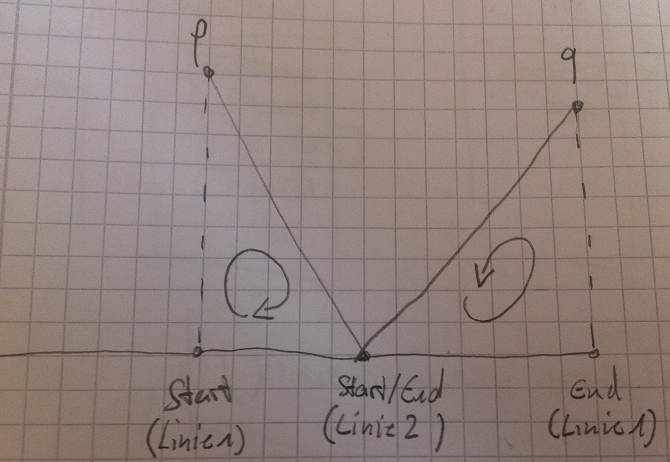
\includegraphics[width=0.7\textwidth]{A1_ccw_kolinier.png}
\caption{Struktur des Tests bei Kolinearität}
\label{fig:A1_kolinear}
\end{figure}

\begin{lstlisting}[captionpos=b, caption={Schnittpunkttest von kolinearen Linien }, label=A1:Kolinear]
...
else { //überlappungstest (line <-> line oder line <-> punkt)
			 //p über m_start - drehung um -90°, q über m_end - drehung um 90° des gegengesetzten Vektor
		Point p(m_end.get_y()-m_start.get_y(), m_end.get_x()-m_start.get_x()),
				  q(m_start.get_y()-m_end.get_y(), m_end.get_x()-m_start.get_x());

		//Start-Punkt auf der Linie (inkl Ränder)
		if( ccw_max(m_start, a_line->m_start, p)*ccw_max(m_end,q,a_line->m_start) >= 0 ){
			return true;
		}
		//End-Punkt auf der Linie (inkl Ränder)
		else if(ccw_max(m_start, a_line->m_end, p)*ccw_max(m_end,q,a_line->m_end) >= 0){
			return true;
		}
		else
			return false;
	}
}
...
\end{lstlisting}

\subsubsection{Normaler Schnittpunkt}
Falls die beiden Strecken nicht auf der selben Gerade liegen, muss lediglich überprüft werden ob die beiden Punkte des einen Segments je auf verschiedenen Seiten der anderen Linie liegen. Dies kann wiederum mit der ccw-Funktion getestet werden. Die Betrachtung wird aus Sicht beider Linien gemacht, sonst würde eine seitlich versetzte Linie als Schnittpunkt gezählt.

\begin{lstlisting}[captionpos=b, caption={Schnittpr\"ufung mit ccw-Funktion}, label=A1:Schnittpunkt]
...
else if ( (ccw_max(m_start, m_end, a_line->m_start)*ccw_max(m_start, m_end, a_line->m_end)) < 0
		  && ccw_max(a_line->m_start, a_line->m_end, m_start)*ccw_max(a_line->m_start, a_line->m_end, m_end) < 0 ) {

	//->Schnittpunkt!!
	return true;
}
return false;
\end{lstlisting}
 
Sind beide Tests negativ, gibt es keinen Schnittpunkt. Es kann also ein sonst generell gültiger Else-Fall erstellt werden, der false zurück liefert.


